\documentclass[11pt,a4paper]{article}
\usepackage[margin=24mm,headheight=15pt]{geometry}
\usepackage[T1]{fontenc}
\usepackage{lmodern,microtype}
\usepackage{amsmath,amssymb,mathtools}
\usepackage{graphicx,tikz,pgfplots}
\usepackage[section]{placeins}
\usetikzlibrary{arrows.meta,positioning,calc}
\pgfplotsset{compat=1.18}
\usepackage{booktabs,tabularx,enumitem}
\usepackage{xcolor,fancyhdr,titlesec}
\definecolor{ink}{HTML}{17324D}
\definecolor{teal}{HTML}{087F8C}
\definecolor{orange}{HTML}{BD622A}
\definecolor{muted}{HTML}{526575}
\usepackage[colorlinks=true,linkcolor=teal,urlcolor=teal,citecolor=teal]{hyperref}
\usepackage{xcolor}
\usepackage{soul}

\newcommand{\note}[1]{%
  \begingroup
  \sethlcolor{yellow}%
  \hl{\textbf{ED:} #1}%
  \endgroup
}
\hypersetup{pdftitle={Quantum Error Correction},pdfauthor={}}
\newcommand{\ket}[1]{\lvert #1\rangle}
\newcommand{\bra}[1]{\langle #1\rvert}
\newcommand{\ii}{\mathrm{i}}
\newcommand{\Prob}{\mathop{\mathrm{P}}}
\newcommand{\id}{\mathbb I}
\newcommand{\wt}{\operatorname{wt}}
\newcommand{\cnot}{\operatorname{CNOT}}
\setlength{\parindent}{0pt}
\setlength{\parskip}{5pt}
\setlength{\emergencystretch}{2em}
\titleformat{\section}{\Large\bfseries\color{ink}}{\thesection}{0.6em}{}
\titleformat{\subsection}{\large\bfseries\color{ink}}{\thesubsection}{0.6em}{}
\pagestyle{fancy}\fancyhf{}
\fancyhead[L]{\small\color{muted} QUANTUM COMPUTING / FOUNDATIONS}
\fancyfoot[L]{\small\color{muted} Tutorial 02: Quantum Error Correction}
\fancyfoot[R]{\small\thepage}
\renewcommand{\headrulewidth}{0.3pt}
\setlist[itemize]{nosep,leftmargin=1.5em}
\setlist[enumerate]{itemsep=3pt,leftmargin=1.5em}
\newcommand{\takeaway}[1]{\begin{quote}\color{ink}\textbf{#1}\end{quote}}
\tikzset{gate/.style={draw=teal,fill=white,minimum width=8mm,minimum height=7mm},measure/.style={draw=ink,fill=white,minimum width=10mm,minimum height=7mm},wire/.style={draw=ink},every picture/.style={>=Latex}}
\newcommand{\ctrl}[2]{\fill[ink] (#1,#2) circle (2pt);}
\newcommand{\targ}[2]{\draw[ink,fill=white] (#1,#2) circle (0.12);\draw[ink] (#1-0.12,#2)--(#1+0.12,#2);\draw[ink] (#1,#2-0.12)--(#1,#2+0.12);}
\begin{document}
\begin{center}
{\small\color{teal}\textbf{PART OF A SERIES OF TUTORIALS ON QUANTUM ERROR CORRECTION}}\\[9pt]
{\LARGE\bfseries\color{ink} Quantum Error Correction}\\[10pt]
{\large From parity checks to a quantum memory experiment}\\[9pt]
{\small Revised 21 September 2026}
\end{center}
\vspace{3pt}
In the previous tutorial, we introduced quantum computing as a way of processing information using the laws of quantum mechanics. We also discussed four central features of quantum information: superposition, interference, entanglement, and measurement. These ideas provide the foundation for understanding quantum error correction, which is essential for building large-scale, fault-tolerant quantum computers.

The primary goal of this tutorial is to introduce stabilizers, error syndromes, and decoding, using the three-qubit repetition code as a running example. We begin with ideal encoding and stabilizer measurements, and then add the complications that arise in practice: errors in the data, noisy measurement outcomes, and faults in the circuits used to extract the syndrome.

\section{Error correction}
When we store or transmit information, errors can happen. Physical noise can change the value read from a bit: a 0 becomes a 1, or a 1 becomes a 0. Our goal is to recover the original message despite these changes.

The basic strategy is \emph{redundancy}: extra bits that do not carry new independent message content but give us a way to recognize and recover from some changes in the original message. Those extra bits might be copies, or they might record relationships among message bits. 

The simplest example is the three-bit repetition code:
\begin{equation}\label{eq:classical-code}
0\longmapsto 000,\qquad 1\longmapsto 111.
\end{equation}

The bit strings \(000\) and \(111\) are the valid \emph{codewords}; each represents one legitimate message, \(0\) or \(1\). If we receive a string such as \(010\), which violates the code's pattern, this may indicate that an error has occurred.
The map from the original bit to its codeword is called \emph{encoding}. After transmission, we apply a \emph{decoding} rule to the received word to infer the original bit. For this code, the decoding rule is majority voting. For example, for the received word \(010\), the majority value is \(0\), so we decode it as \(0\). Assuming that at most one bit has flipped, we infer that the middle bit was faulty. We can then correct the received word by flipping that bit, recovering the codeword \(000\), which represents the original message \(0\).
None of the three bits is a guaranteed reference; we trust the majority because of our assumption about the error process.

If each bit flips independently with probability \(p\), and all other operations are ideal, majority voting fails whenever at least two of the three bits are flipped:
\begin{equation}\label{eq:classical-failure}
P_{\mathrm{fail}}
= \binom{3}{2}p^2(1-p)+p^3
= 3p^2-2p^3 .
\end{equation}

For \(0<p<\tfrac12\), we have \(P_{\mathrm{fail}}<p\). Thus, under this independent-error model, the three-bit repetition code reduces the probability of an incorrect decoded bit. At \(p=\tfrac12\), encoding provides no improvement; for \(\tfrac12<p<1\), the decoded bit is more likely to be wrong than the original unencoded bit. The assumptions matter: for example, a disturbance that flips all three bits defeats majority voting. We will later consider errors in the checking and decoding processes themselves.

\subsection{Parity: checking a relationship}
How do we compare the copies? XOR, written $\oplus$, returns 0 when two bits agree and 1 when they disagree:
\[
0\oplus0=1\oplus1=0,\qquad 0\oplus1=1\oplus0=1.
\]
For three bits $b_1b_2b_3$, define two parity checks:
\begin{equation}\label{eq:classical-checks}
s_1=b_1\oplus b_2,\qquad s_2=b_2\oplus b_3.
\end{equation}
The pair of check outcomes $s_1s_2$ is called the \emph{syndrome}. Both valid codewords, $000$ and $111$, give $s_1s_2=00$.
For a single-bit error, the syndrome identifies which check was
violated. If bit \(1\) flips, only the first check changes, giving
\(s_1s_2=10\). If bit \(2\) flips, both checks change, giving
\(s_1s_2=11\). If bit \(3\) flips, only the second check changes,
giving \(s_1s_2=01\), regardless of the original codeword being \(000\) or \(111\). Thus, the checks reveal where the bits disagree, but not whether the original message was \(0\) or \(1\).

\begin{figure}[!ht]
\centering
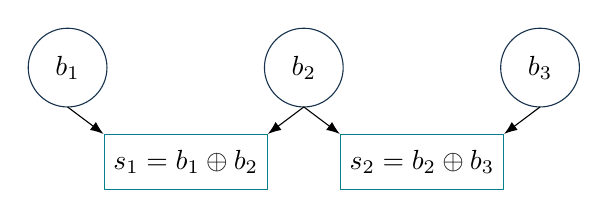
\begin{tikzpicture}
\foreach \x/\lab in {0/b_1,3/b_2,6/b_3}{\node[draw=ink,circle,minimum size=10mm] at (\x,0) {$\lab$};}
\node[gate] (s1) at (1.5,-1.2) {$s_1=b_1\oplus b_2$};
\node[gate] (s2) at (4.5,-1.2) {$s_2=b_2\oplus b_3$};
\draw[->] (0,-.5)--(s1.north west);\draw[->] (3,-.5)--(s1.north east);
\draw[->] (3,-.5)--(s2.north west);\draw[->] (6,-.5)--(s2.north east);
\end{tikzpicture}
\caption{The middle bit participates in both checks. A single flip there changes both check outcomes. A boundary bit participates in only one check.}
\end{figure}

Replication and parity checks are not competing ideas: replication supplies redundancy, and parity checks test its structure. Other codes use parity bits instead of literal copies. For example, append $p=b_1\oplus b_2\oplus b_3$, so every valid encoded string satisfies $b_1\oplus b_2\oplus b_3\oplus p=0$. An odd total parity detects an error, but one check cannot locate it, and an even number of flips can go unnoticed. Carefully chosen overlapping checks can identify errors with less redundancy than repetition.

\takeaway{A code can be described by its valid messages, or by the constraints those messages must satisfy. This second viewpoint is the bridge to quantum error correction.}

\newpage
\section{Quantum errors: bits, phases, and small rotations}
For a qubit, preserving the values \(0\) and \(1\) is not enough. We
must also preserve the amplitudes and their relative phase. The
single-qubit Pauli operators provide a useful language for describing
the most important errors:
\begin{equation}
I=\begin{pmatrix}1&0\\0&1\end{pmatrix},\quad
X=\begin{pmatrix}0&1\\1&0\end{pmatrix},\quad
Y=\begin{pmatrix}0&-\ii\\\ii&0\end{pmatrix},\quad
Z=\begin{pmatrix}1&0\\0&-1\end{pmatrix}.
\end{equation}
Their algebra includes
\begin{equation}\label{eq:pauli-algebra}
X^2=Z^2=I,\qquad XZ=-ZX,\qquad Y=\ii XZ.
\end{equation}

The square of each Pauli operator becomes the identity; distinct nonidentity single-qubit Paulis anticommute; the product of two
distinct nonidentity Pauli operators is proportional to the remaining
one. Since \(Y\) is, up to a phase, a product of \(X\) and
\(Z\), we can use \(X\) and \(Z\) as the two basic error types.
For $\ket{\psi}=\alpha\ket0+\beta\ket1$,
\begin{align}
X\ket\psi&=\alpha\ket1+\beta\ket0,\label{eq:x-error}\\
Z\ket\psi&=\alpha\ket0-\beta\ket1.\label{eq:z-error}
\end{align}
We call $X$ a bit flip and $Z$ a phase flip, relative to the computational basis. 

In the Bloch-sphere representation, each of \(X\), \(Y\), and \(Z\)
acts as a \(180^\circ\) rotation---a half-turn---about its corresponding
axis. In particular, \(X\) exchanges \(\ket{0}\) and \(\ket{1}\).
The operator \(Y\) is, up to an overall phase, equivalent to applying
\(Z\) and \(X\) in succession.

\subsection{What if the error is only a small rotation?}
Physical errors need not be exact half-turns. Since $X^2=I$, expanding the exponential separates its even and odd powers:
\begin{equation}\label{eq:rotation}
R_X(\epsilon)=e^{-\ii\epsilon X/2}
=\cos\frac\epsilon2 I-\ii\sin\frac\epsilon2 X.
\end{equation}
A small rotation is a coherent linear combination of $I$ and $X$, not necessarily a random choice between them. More generally, every single-qubit operator expands in $I,X,Y,Z$. This is why Pauli errors are useful building blocks even for continuous noise. Once we have a code and a syndrome measurement, we will show exactly how Eq.~\eqref{eq:rotation} can be corrected.

\subsection{What about entangled, multi-qubit states?}
An entangled state cannot be represented by separate pure-state Bloch spheres, but Pauli operators still work. On $n$ qubits we use \emph{Pauli strings}, such as $X\otimes I\otimes Z$, and every operator has an expansion
\begin{equation}\label{eq:pauli-expansion}
E=\sum_{P\in\{I,X,Y,Z\}^{\otimes n}}c_P P.
\end{equation}
There are $4^n$ such basis operators. They act on entangled states just as on any other state: for example, $(X\otimes I)(\ket{00}+\ket{11})/\sqrt2=(\ket{10}+\ket{01})/\sqrt2$. For general open-system noise, each Kraus operator has a Pauli expansion; a general channel need not be a classical mixture of Pauli errors.

\newpage
\section{Defining a quantum code through stabilizers}
A code can be described by its valid codewords or by the constraints they must satisfy. For a quantum code, superpositions of its basis codewords must also be valid. Error correction must preserve these superpositions: a measurement that identifies the logical codeword would collapse the encoded state and destroy the coherence we want to protect. We therefore check constraints shared by all valid code states. \emph{Stabilizer codes} provide such checks, extending classical parity checks to quantum information and giving us the language used later for the surface code.

We choose mutually commuting Hermitian Pauli operators \(S_1,\ldots,S_r\), called \emph{stabilizer generators}.\footnote{Hermitian means \(A=A^\dagger\), where \(\dagger\) is the conjugate transpose. Such operators represent observables and have real eigenvalues. Tensor products of \(I,X,Y,Z\), with an overall sign \(\pm1\), are Hermitian; the full Pauli group also includes factors \(\pm\ii\), which are not suitable as observables. A nonidentity Hermitian Pauli check has outcomes \(+1\) and \(-1\).}
Their products, including the identity, form the \emph{stabilizer group} \(\mathcal S=\langle S_1,\ldots,S_r\rangle\).
The \emph{codespace} consists of the states that every element of this group leaves unchanged:
\begin{equation}\label{eq:codespace}
S\ket{\psi_L}=\ket{\psi_L}\qquad\text{for every }S\in\mathcal S.
\end{equation}
Equivalently, it is their common \(+1\) eigenspace. Measuring a generator returns \(+1\) for a satisfied check and \(-1\) for a violated check. Commutation makes the checks compatible. We also require \(-I\notin\mathcal S\): otherwise the constraints would demand \(-\ket{\psi_L}=\ket{\psi_L}\), which no nonzero state can satisfy. The identity \(I\), in contrast, always belongs to the group. Stabilizer codes are one class of quantum codes, not the only possibility \cite{ibm-stabilizers}.

\subsection{The repetition code as quantum parity checks}
For a computational-basis bit \(b\), \(Z\ket b=(-1)^b\ket b\). Consequently,
\begin{equation}
(Z\otimes Z)\ket{b_1b_2}=(-1)^{b_1+b_2}\ket{b_1b_2}.
\end{equation}
Thus \(ZZ\) has eigenvalue \(+1\) when the two bits agree and \(-1\) when they disagree. On three qubits, choose
\begin{equation}\label{eq:generators}
S_1=Z_1Z_2=ZZI,\qquad S_2=Z_2Z_3=IZZ,\qquad
\mathcal S=\{III,ZZI,IZZ,ZIZ\}.
\end{equation}
Here \(Z_j\) means \(Z\) on qubit \(j\) and identity elsewhere; adjacent letters denote tensor products. There are two independent generators: the third nonidentity stabilizer, \(ZIZ=S_1S_2\), adds no new constraint.

Both checks require adjacent bits to agree, so the only allowed computational-basis strings are \(000\) and \(111\). We identify \(\ket{0_L}=\ket{000}\) and \(\ket{1_L}=\ket{111}\), where \(L\) denotes a \emph{logical} qubit encoded across the three physical qubits. By linearity, every normalized superposition
\begin{equation}\label{eq:logical-basis}
\ket{\psi_L}=\alpha\ket{000}+\beta\ket{111}
\end{equation}
passes both checks, whatever the amplitudes \(\alpha\) and \(\beta\).

A single \(X\) error breaks one or both of these parity constraints. A \(Z\) error commutes with both checks and can change the logical relative phase undetected. To detect phase flips instead, use the same construction in the \(X\) basis: the checks \(X_1X_2\) and \(X_2X_3\) stabilize all superpositions of \(\ket{+++}\) and \(\ket{---}\). Since \(Z\ket+=\ket-\) and \(Z\ket-=\ket+\), a \(Z\) error now creates a disagreement. This phase-flip code has the complementary vulnerability to \(X\) errors. Protecting against both requires a different code with suitable compatible checks; we cannot simply combine these two sets, since some of their checks anticommute.

\newpage
\section{Syndromes: reading the checks}
The measured check outcomes form a \emph{syndrome}, just as in the classical code. We record \(+1\) as bit \(0\) and \(-1\) as bit \(1\). A valid code state gives the trivial syndrome \(00\cdots0\). To see how an error changes it, recall that two Pauli strings either commute or anticommute. For a Pauli error \(E\),
\begin{equation}\label{eq:syndrome-sign}
S_iE=(-1)^{s_i(E)}ES_i
\quad\Longrightarrow\quad
S_iE\ket{\psi_L}=(-1)^{s_i(E)}E\ket{\psi_L}.
\end{equation}
A commuting error leaves that check at \(+1\); an anticommuting error changes it to \(-1\). For example, \(X_2\) anticommutes with both \(Z_1Z_2\) and \(Z_2Z_3\), giving syndrome \(11\). The complete single-flip pattern is compact:
\begin{equation}
I\longrightarrow00,\qquad X_1\longrightarrow10,\qquad
X_2\longrightarrow11,\qquad X_3\longrightarrow01.
\end{equation}
If at most one \(X\) error occurred before an ideal check round, the syndrome identifies it. Applying the same \(X_j\) again restores the encoded state because \(X_j^2=I\). The sign in Eq.~\eqref{eq:syndrome-sign} depends on the error and the check, not on \(\alpha\) or \(\beta\): we learn about the error without learning the message.

\subsection{What the syndrome does not tell us}
A \emph{decoder} uses the syndrome and an error model to choose a recovery. The syndrome alone need not identify a unique error: \(X_1\) and \(X_2X_3\) both give \(10\). If we assume a single flip and apply \(X_1\) when the actual error was \(X_2X_3\), the remaining operation is \(X_1X_2X_3\). It exchanges the two valid codewords, so the checks pass even though the logical information has changed.

Likewise, syndrome \(00\) means that no check was violated, not that no error occurred. Recovery succeeds when the combined error and correction leave \emph{every} encoded state unchanged, up to a global phase. We do not need to identify the exact physical error if several possible errors have the same effect on the encoded information. To make this distinction precise, we need logical operators.

\section{Logical operators: changing the encoded information}
Stabilizers leave every code state unchanged. A \emph{logical operator} keeps the state inside the codespace while acting on the encoded information. For a Pauli operator \(L\) that commutes with every check,
\begin{equation}
S_iL\ket{\psi_L}=LS_i\ket{\psi_L}=L\ket{\psi_L}.
\end{equation}
Thus the state still passes every check. If \(L\) is a stabilizer, it does nothing to the encoded information. If it is not proportional to a stabilizer, it implements a nontrivial logical Pauli.

For the repetition code, we choose
\begin{equation}\label{eq:logical-paulis}
\overline X=X_1X_2X_3,\qquad \overline Z=Z_1.
\end{equation}
The first exchanges \(\ket{0_L}\) and \(\ket{1_L}\); the second leaves \(\ket{0_L}\) unchanged and multiplies \(\ket{1_L}\) by \(-1\). They act just like \(X\) and \(Z\) on one qubit. Both commute with the stabilizers, but they anticommute with each other: \(\overline X\overline Z=-\overline Z\overline X\).

Fixing one particular code state is not enough to make an operator a stabilizer. For example, \(Z_1\) fixes \(\ket{0_L}\), but changes \((\ket{0_L}+\ket{1_L})/\sqrt2\). The distinction is its action on the \emph{whole codespace}. Logical representatives are also not unique: \(Z_2=Z_1S_1\), so \(Z_1\) and \(Z_2\) have the same logical action. More generally, multiplying by a stabilizer does not change that action.

Could we choose \(Z_1\) as an additional stabilizer? Yes, but then only multiples of \(\ket{000}\) pass all three checks. We have fixed the logical value and lost the freedom to encode an arbitrary qubit. This gives us a way to count how much information a code can hold.

\subsection{Counting information and protection: \texorpdfstring{\([[n,k,d]]\)}{[[n,k,d]]}}
An \(n\)-qubit register has \(2^n\) independent basis states. Each independent, consistent Pauli check halves the dimension available to the code. With \(r\) independent generators, the remaining dimension is \(2^{n-r}\), enough to encode \(k=n-r\) logical qubits:
\begin{equation}\label{eq:count}
\dim\mathcal C=2^{n-r}=2^k,\qquad r=n-k.
\end{equation}
Our two checks on three qubits therefore leave one logical qubit. In general, the stabilizer group has \(2^{n-k}\) elements, while the logical Pauli operators are generated by \(k\) pairs \((\overline X_j,\overline Z_j)\). Each pair anticommutes; operators for different logical qubits commute. Ignoring global phases and identifying representatives that differ by a stabilizer gives \(4^k\) logical Pauli classes.

To describe protection as well as capacity, we write \([[n,k,d]]\). Here \(n\) counts physical data qubits, \(k\) counts encoded logical qubits, and the \emph{distance} \(d\) is the smallest number of qubits on which a Pauli error can act to make an undetected logical change:
\begin{equation}\label{eq:distance}
d=\min_{L\text{ nontrivial logical Pauli}}\wt(L).
\end{equation}
The weight counts nonidentity factors: \(\wt(XII)=1\) and \(\wt(XZX)=3\). A low-weight stabilizer does not reduce the distance because it leaves the encoded information unchanged.

Two Pauli errors, each affecting at most \(t\) qubits, differ by an operator of weight at most \(2t\). If \(2t<d\), they cannot have both the same syndrome and different logical effects. This is why a distance-\(d\) code, with ideal recovery, corrects arbitrary errors on up to \(t=\lfloor(d-1)/2\rfloor\) qubits \cite{gottesman}.

The repetition code is \([[3,1,1]]\): \(Z_1\) is already a weight-one logical error. Its protection against one \(X\) error does not imply protection against every single-qubit error. The smallest purely \(X\) logical operator has weight three, explaining that restricted protection. Measurement ancillas are additional hardware and are not counted in \(n\).

\section{Returning to small rotations}
We can now answer the question from Eq.~\eqref{eq:rotation}. A small rotation on the first data qubit gives
\begin{equation}
R_{X_1}(\epsilon)\ket{\psi_L}
=\cos\frac{\epsilon}{2}\ket{\psi_L}
-\ii\sin\frac{\epsilon}{2}X_1\ket{\psi_L}.
\end{equation}
The two terms have different syndromes. Ideal check measurements return \(00\) with probability \(\cos^2(\epsilon/2)\), leaving the original encoded state, or \(10\) with probability \(\sin^2(\epsilon/2)\), leaving \(X_1\ket{\psi_L}\) up to a global phase. In the latter case, applying \(X_1\) restores the state. We do not need to estimate the rotation angle.

This works because both components are correctable. A rotation generated by \(Z_1=\overline Z\), however, changes the logical relative phase while leaving every check satisfied. More generally, a code that corrects a set of errors also corrects their linear combinations. Syndrome measurement separates components with different syndromes; it does not imply that the original noise was a random choice of Pauli errors \cite{ibm-errors}.

We have described what the checks reveal. Next we need circuits that obtain that information while preserving the encoded superposition.

\newpage
\section{Implementation: a three-qubit quantum memory}\label{sec:implementation}

We have described how the repetition code detects and corrects a
single bit flip. Now we want to implement this protection: prepare one
logical qubit, store it while repeatedly checking for errors, and
finally read out its logical value. Our three data qubits are checked
by \(S_1=Z_1Z_2\) and \(S_2=Z_2Z_3\). Additional qubits, called
\emph{ancillas}, let us read these checks without directly measuring
the encoded information.

\subsection{From CNOT gates to a parity check}

The controlled-NOT gate, or CNOT, has a control qubit \(c\) and a
target qubit \(t\). It flips the target when the control is
\(\ket1\):
\begin{equation}
\cnot_{c\to t}\ket{x}_c\ket{y}_t
=\ket{x}_c\ket{y\oplus x}_t.
\end{equation}
Its action on superpositions follows by linearity. In circuit
diagrams, the filled dot marks the control and the circled plus marks
the target; time runs from left to right.

To measure \(Z_1Z_2\), prepare an ancilla in \(\ket0\), apply a CNOT
from each data qubit to the ancilla, and then measure the ancilla in
the computational basis:
\begin{equation}\label{eq:zz-extraction}
\ket{b_1b_2}\ket0_a
\xrightarrow{\mathrm{CNOT}_{1\to a}}
\ket{b_1b_2}\ket{b_1}_a
\xrightarrow{\mathrm{CNOT}_{2\to a}}
\ket{b_1b_2}\ket{b_1\oplus b_2}_a.
\end{equation}
Measuring the ancilla in the computational basis then gives
\(m=b_1\oplus b_2\), corresponding to the check eigenvalue
\(\lambda=(-1)^m\).


The shared ancilla implements the selective readout we need: \(00\)
and \(11\) leave it in the same state, as do \(01\) and \(10\).
Measuring it distinguishes the two parities while preserving
superpositions within each parity sector. Both CNOTs must precede
the measurement; reading the ancilla after only the first would
reveal the individual value \(b_1\).

The \(Z_2Z_3\) check uses the same circuit with data qubits \(2\)
and \(3\). Together, the two check results form one syndrome round;
each ancilla must be prepared in \(\ket0\) before its next use.

We can also track the measured observable. With
\(U=\cnot_{2\to a}\cnot_{1\to a}\),
\begin{equation}
U^\dagger Z_aU=Z_1Z_2Z_a.
\end{equation}
Since the input ancilla has \(Z_a=+1\), measuring its output reads
the data observable \(Z_1Z_2\). This is the Heisenberg viewpoint:
follow the observable through the circuit rather than the state.

\subsection{Detecting phase errors with an X check}
The same idea detects phase errors, but the check basis is reversed. A
$Z$ error changes a relative phase and can commute with the $Z$ checks
of the bit-flip repetition code. To detect it, use the phase-flip code
with checks $X_1X_2$ and $X_2X_3$. A $Z$ error anticommutes with every
$X$ check that contains its qubit, so it changes the corresponding
syndrome signs.

The encoded state here is $\alpha\ket{+++}+\beta\ket{---}$.
This is a different encoding from $\alpha\ket{000}+\beta\ket{111}$:
we have changed the basis of the entire code, not added an incompatible
check to the old code.

The two circuits make the basis reversal visible. A $Z$ check detects
bit flips: the data qubits control CNOTs into a $\ket0$ ancilla, which
is then read in $Z$. An $X$ check detects phase flips: a $\ket+$ ancilla
controls the CNOTs into the data, and is read in $X$. In both cases the
ancilla reveals only the two-qubit parity.

\begin{figure}[!ht]
\centering
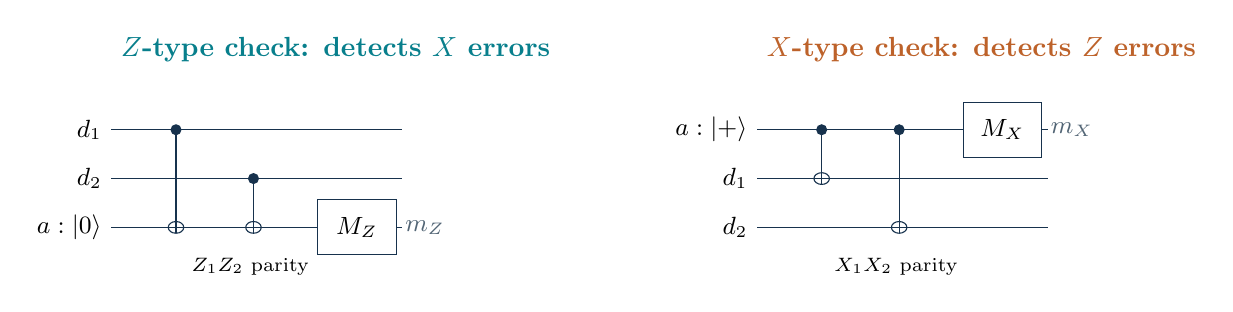
\begin{tikzpicture}[x=.82cm,y=.62cm,font=\small]
  % Z-type check
  \begin{scope}
    \node[anchor=west,font=\bfseries,text=teal] at (0,1.65) {$Z$-type check: detects $X$ errors};
    \foreach \y/\name in {0/{d_1},-1/{d_2},-2/{a:\ket0}} {
      \draw[wire] (0,\y)--(4.5,\y);
      \node[anchor=east] at (0,\y) {$\name$};
    }
    \draw[ink] (1,0)--(1,-2); \ctrl{1}{0}\targ{1}{-2}
    \draw[ink] (2.2,-1)--(2.2,-2); \ctrl{2.2}{-1}\targ{2.2}{-2}
    \node[measure] at (3.8,-2) {$M_Z$};
    \node[anchor=west,text=muted] at (4.4,-2) {$m_Z$};
    \node[align=center,font=\scriptsize] at (2.15,-2.8) {$Z_1Z_2$ parity};
  \end{scope}
  % X-type check
  \begin{scope}[xshift=8.2cm]
    \node[anchor=west,font=\bfseries,text=orange] at (0,1.65) {$X$-type check: detects $Z$ errors};
    \foreach \y/\name in {0/{a:\ket+},-1/{d_1},-2/{d_2}} {
      \draw[wire] (0,\y)--(4.5,\y);
      \node[anchor=east] at (0,\y) {$\name$};
    }
    \draw[ink] (1,0)--(1,-1); \ctrl{1}{0}\targ{1}{-1}
    \draw[ink] (2.2,0)--(2.2,-2); \ctrl{2.2}{0}\targ{2.2}{-2}
    \node[measure] at (3.8,0) {$M_X$};
    \node[anchor=west,text=muted] at (4.4,0) {$m_X$};
    \node[align=center,font=\scriptsize] at (2.15,-2.8) {$X_1X_2$ parity};
  \end{scope}
\end{tikzpicture}
\caption{The same parity-measurement pattern in two complementary bases. Filled dots are CNOT controls and circled pluses are targets. The direction of each CNOT, the prepared ancilla state, and the readout basis all reverse together.}
\label{fig:check-bases}
\end{figure}

To measure $X_1X_2$, prepare an ancilla in $\ket{+}$, use it as the
control of CNOTs targeting data qubits 1 and 2, and measure the ancilla
in the $X$ basis. If $U$ is this two-CNOT circuit, then
\[
U^\dagger X_aU=X_aX_1X_2.
\]
Because the input ancilla has $X_a=+1$, its final $X$ readout measures
$X_1X_2$. Equivalently, apply $H$ to the ancilla and measure it in the
computational basis. The syndrome table is the phase analogue of the
one above:
\[
I\longrightarrow00,\qquad Z_1\longrightarrow10,\qquad
Z_2\longrightarrow11,\qquad Z_3\longrightarrow01.
\]
For example, $Z_2$ anticommutes with both $X_1X_2$ and $X_2X_3$, so both
check outcomes flip. Applying the inferred $Z_2$ restores the encoded
state. The bit-flip and phase-flip repetition codes are complementary;
their checks cannot simply be combined because some $X$-type and
$Z$-type checks would anticommute. A full quantum code must choose a
larger compatible set of checks, as the surface code does.

\subsection{Preparing the logical state}

To encode \(\ket\psi=\alpha\ket0+\beta\ket1\), initialize the other
two data qubits in \(\ket0\) and apply CNOTs from qubit \(1\) to
qubits \(2\) and \(3\):
\begin{equation}
\begin{aligned}
(\alpha\ket0+\beta\ket1)\ket{00}
&\xrightarrow{\cnot_{1\to2}}
\alpha\ket{000}+\beta\ket{110}\\
&\xrightarrow{\cnot_{1\to3}}
\alpha\ket{000}+\beta\ket{111}
=\ket{\psi_L}.
\end{aligned}
\end{equation}
All three output qubits now store the logical information. This
does not create three independent copies of \(\ket\psi\); it
encodes the state in their joint state.

For a first memory experiment, we can prepare \(\ket{0_L}\) or
\(\ket{1_L}\) simply by preparing \(\ket{000}\) or \(\ket{111}\).
To prepare \(\ket{+_L}\), use \(\ket+\) as the input to the
encoding circuit. We initially assume ideal preparation; the
encoding circuit alone does not guarantee protection against faults
during preparation.

\subsection{Noisy checks and a memory experiment}\label{sec:memory}

In practice, the checking circuit can also fail. An ancilla readout
may report the wrong bit, and a faulty gate may affect the data,
the ancilla, or both. One unexpected syndrome therefore need not
mean that a data qubit flipped. We repeat the checks and use their
history to distinguish likely explanations.

First consider a simple model: data \(X\) errors occur between ideal
rounds, and reported syndrome bits can be wrong. If no corrections
are applied between rounds, a persistent parity change might produce
\(0,0,1,1,1\), whereas one bad report might produce \(0,0,1,0,0\).
The difference is visible in the changes between consecutive results:
\begin{equation}
\delta_i(t)=\widetilde s_i(t)\oplus\widetilde s_i(t-1),
\end{equation}
where \(\widetilde s_i(t)\) is the recorded result of check \(i\)
in round \(t\). This parity is a detector outcome; a nonzero outcome is a \emph{detection event}.
A decoder uses their pattern across checks and time, together with
an error model, to infer a recovery. A detailed circuit-noise model
must also account for faults during the CNOTs.

A memory experiment follows this sequence: prepare a logical state,
store it through \(T\) rounds of checks, then measure the data and
decode the complete record. We need not physically correct the data
after every round; inferred Pauli corrections can be tracked
classically and included when interpreting the final readout.

\subsection{Reading the logical information}

At the end of storage or computation, we deliberately read the
encoded information. The measurement basis selects a logical
observable; this final readout need not preserve the encoded state.

For logical \(Z\), measure all three data qubits in \(Z\). With ideal
checks and at most one flip in the final three-bit record, majority
voting gives the logical bit. With noisy repeated checks, the decoder
uses the syndrome history together with these final outcomes.
For an undamaged state
\(\alpha\ket{0_L}+\beta\ket{1_L}\), the logical outcomes \(0\) and \(1\)
have probabilities \(|\alpha|^2\) and \(|\beta|^2\).

For logical \(X\), use \(\overline X=X_1X_2X_3\): measure each data
qubit in \(X\) and multiply the three eigenvalue outcomes.
Equivalently, apply \(H\) to each qubit before a \(Z\) measurement.
If the resulting bits are \(b_1,b_2,b_3\), the logical eigenvalue is
\begin{equation}
\overline x=(-1)^{b_1+b_2+b_3}.
\end{equation}
Unlike the majority-vote readout, one incorrect individual outcome
flips this product. The repetition code does not protect both
logical observables equally.

To assess the memory, repeat the experiment and compare the decoded
logical result with the prepared value. Preparing and reading only
\(\ket{0_L}\) and \(\ket{1_L}\) tests preservation of a logical bit;
it does not establish preservation of an arbitrary quantum state.
The undetected phase errors of this code remain the reason we need
codes that protect against both bit and phase errors.

\begin{figure}[!ht]
\centering
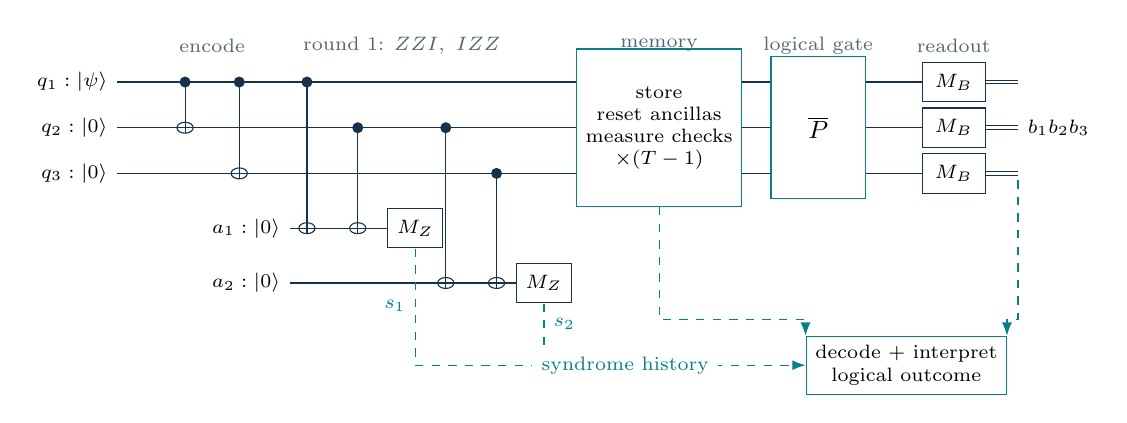
\begin{tikzpicture}[x=.86cm,y=.58cm,font=\small]
% Three quantum data wires.
\foreach \y/\lab in {0/{q_1:\ket\psi},-1/{q_2:\ket0},-2/{q_3:\ket0}}{
  \draw[wire] (0,\y)--(12.35,\y);
  \node[left,font=\scriptsize] at (0,\y) {$\lab$};
}
% Encoding.
\draw[ink] (1,0)--(1,-1);\ctrl{1}{0}\targ{1}{-1}
\draw[ink] (1.8,0)--(1.8,-2);\ctrl{1.8}{0}\targ{1.8}{-2}
\node[font=\scriptsize,text=muted] at (1.4,.8) {encode};
% One complete check round, using fresh ancillas.
\node[left,font=\scriptsize] at (2.55,-3.2) {$a_1:\ket0$};
\node[left,font=\scriptsize] at (2.55,-4.4) {$a_2:\ket0$};
\draw[wire] (2.55,-3.2)--(4.4,-3.2);
\draw[wire] (2.55,-4.4)--(6.3,-4.4);
\draw[ink] (2.8,0)--(2.8,-3.2);\ctrl{2.8}{0}\targ{2.8}{-3.2}
\draw[ink] (3.55,-1)--(3.55,-3.2);\ctrl{3.55}{-1}\targ{3.55}{-3.2}
\draw[ink] (4.85,-1)--(4.85,-4.4);\ctrl{4.85}{-1}\targ{4.85}{-4.4}
\draw[ink] (5.6,-2)--(5.6,-4.4);\ctrl{5.6}{-2}\targ{5.6}{-4.4}
\node[measure,minimum width=7mm,minimum height=5mm,font=\scriptsize] at (4.4,-3.2) {$M_Z$};
\node[measure,minimum width=7mm,minimum height=5mm,font=\scriptsize] at (6.3,-4.4) {$M_Z$};
\node[font=\scriptsize,text=muted] at (4.2,.8) {round 1: $ZZI,\ IZZ$};
% Boxed repetition of the extraction procedure; ancillas are internal.
\node[gate,minimum width=20mm,minimum height=20mm,align=center,font=\scriptsize] (repeat) at (8,-1) {store\\reset ancillas\\measure checks\\$\times(T-1)$};
\node[font=\scriptsize,text=muted] at (8,.8) {memory};
% An optional known logical Pauli, preserving the codespace.
\node[gate,minimum width=12mm,minimum height=18mm,align=center] (logical) at (10.35,-1) {$\overline P$};
\node[font=\scriptsize,text=muted] at (10.35,.8) {logical gate};
% Terminal measurement and classical output bundle.
\foreach \y in {0,-1,-2}{
  \draw[wire] (12.35,\y+.04)--(13.3,\y+.04);
  \draw[wire] (12.35,\y-.04)--(13.3,\y-.04);
  \node[measure,minimum width=8mm,minimum height=5mm,font=\scriptsize] at (12.35,\y) {$M_B$};
}
\node[font=\scriptsize,text=muted] at (12.35,.8) {readout};
\node[right,font=\scriptsize] at (13.3,-1) {$b_1b_2b_3$};
% Classical information to the decoder, shown as dashed arrows.
\node[gate,align=center,font=\scriptsize,minimum width=25mm] (decode) at (11.65,-6.2) {decode + interpret\\logical outcome};
\draw[->,dashed,teal] (4.4,-3.65)--(4.4,-6.2)--(decode.west);
\draw[->,dashed,teal] (6.3,-4.85)--(6.3,-6.2);
\node[left,font=\scriptsize,text=teal] at (4.4,-4.9) {$s_1$};
\node[right,font=\scriptsize,text=teal] at (6.3,-5.3) {$s_2$};
\node[font=\scriptsize,fill=white,text=teal] at (7.5,-6.2) {syndrome history};
\draw[->,dashed,teal] (repeat.south)--(8,-5.2)-|(decode.north west);
\draw[->,dashed,teal] (13.3,-2.15)--(13.3,-5.2)-|(decode.north east);
\end{tikzpicture}
\caption{From encoding to logical readout. One explicit check round and \(T-1\) boxed rounds give \(T\) rounds in total. Choose \(\overline P=I\) for a memory experiment, or apply a known logical \(\overline X\) or \(\overline Z\). \(M_B\) measures in \(B=Z\) or \(X\); decoding uses the full record and accounts for \(\overline P\). Double wires and dashed arrows carry classical results. Crossings without dots are not gates.}\label{fig:qec-lifecycle}
\end{figure}

\section{Where this leads: Shor's code and the surface code}
Shor's nine-qubit code is one way to combine bit- and phase-error protection. It corrects any single-qubit error under ideal recovery and provides an optional next example. The next tutorial in this series instead develops the surface code directly.

We then turn to the surface code, where geometry becomes central.
Local \(X\)-type and \(Z\)-type checks are arranged across a
two-dimensional layout. That arrangement determines which errors
affect which checks, how logical operators cross the code, and how
distance grows with its size. The same stabilizer and syndrome
language will let us understand this geometric construction.

\bigskip\hrule\medskip
\textbf{Questions to check your understanding}
\begin{enumerate}
\item Why do parity checks of a repetition code reveal disagreement without revealing the original bit?
\item Why do commuting check operators need the additional condition $-I\notin\mathcal S$?
\item Why is $Z_1$ logical rather than a stabilizer, even though it fixes $\ket{0_L}$?
\item Why does a small $X_1$ rotation have correctable syndrome components, while a small $Z_1$ rotation does not in this code?
\item How does measuring an ancilla implement a $ZZ$ measurement? Which observable do you obtain by tracking its readout backward?
\item What distinguishes a persistent data fault from one bad syndrome report in an idealized time history?
\item What can a logical-$Z$ repetition-code memory experiment establish, and what does it leave untested?
\end{enumerate}

\begin{thebibliography}{9}\small
\bibitem{ibm-stabilizers} IBM Quantum Learning. \href{https://quantum.cloud.ibm.com/learning/en/courses/foundations-of-quantum-error-correction/stabilizer-formalism/stabilizer-codes}{Stabilizer codes.} Definition, consistency conditions, and repetition-code examples.
\bibitem{gottesman} D. Gottesman (1997). \href{https://arxiv.org/abs/quant-ph/9705052}{Stabilizer Codes and Quantum Error Correction.} PhD thesis, arXiv:quant-ph/9705052. A general reference for stabilizer groups, logical operators, and distance.
\bibitem{ibm-errors} IBM Quantum Learning. \href{https://quantum.cloud.ibm.com/learning/en/courses/foundations-of-quantum-error-correction/correcting-quantum-errors/introduction}{Correcting quantum errors: introduction.} Error discretization and the transition to full quantum protection.
\bibitem{ibm-repetition} IBM Quantum Documentation. \href{https://quantum.cloud.ibm.com/docs/en/tutorials/repetition-codes}{Repetition codes.} Ancilla-based syndrome extraction and a memory experiment; note the limits of computational-basis benchmarking.
\end{thebibliography}

\end{document}
